\documentclass{article}

\usepackage[utf8]{inputenc}
\usepackage[english]{babel}
\usepackage{multicol} % Allows 2 columns
\usepackage[margin=0.5cm]{geometry} % Set the margin on the sides of the page
\usepackage[dvipsnames]{xcolor} % Allows changing colours oftext and page
\usepackage{graphicx} % Allows importing of pictures
\usepackage{tgheros} % Sets font

\definecolor{backgroundColour}{RGB}{4, 2, 9} % Defines the page colour

\pagecolor{backgroundColour} % Changes the page colour
\color{white} % Changes the text colour

\begin{document}

\begin{center} % Make the title massive
    \begin{Huge}
        Dead Air\\
    \end{Huge}    
    A narrative phone dialling simulator by Matthew Shaw
\end{center}


\begin{multicols}{2}
    %Everything in this section will be in the first column
    
    \begin{center}
        \includegraphics[width=10cm]{Img1}\\
        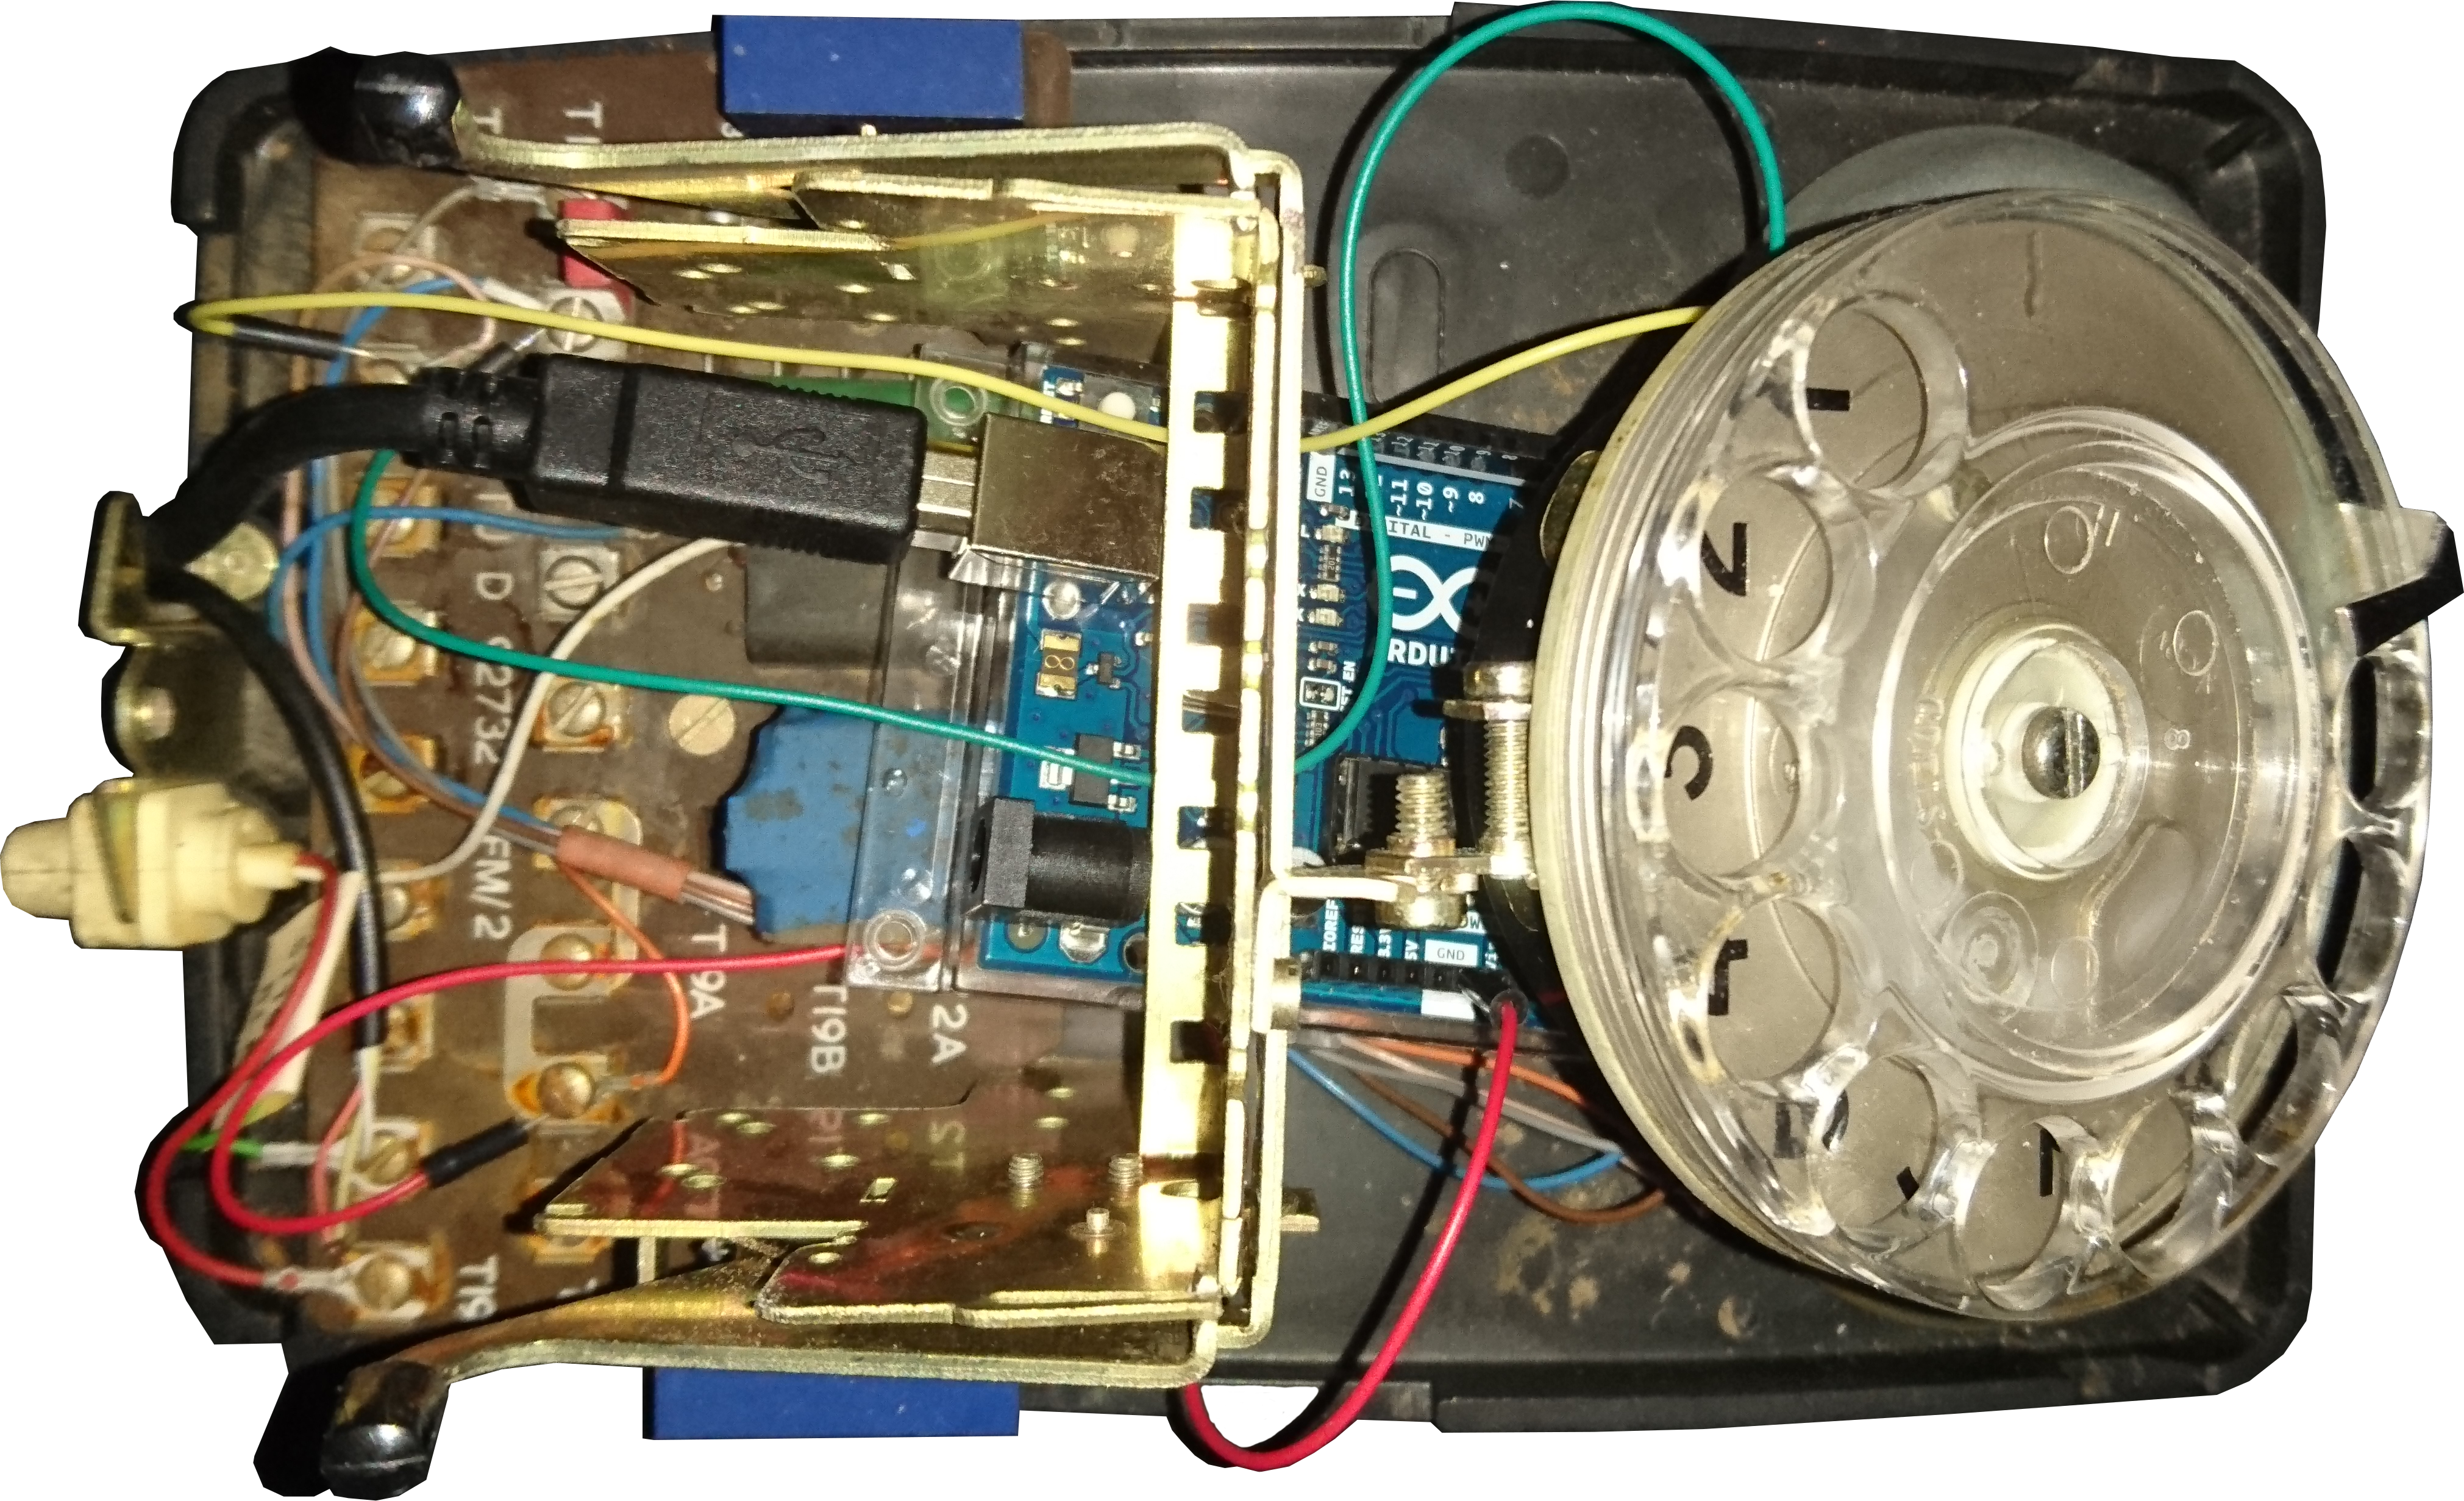
\includegraphics[width=8cm, angle=90]{Img2}\\
        \includegraphics[width=7.5cm]{CircuitDiagramDark}\\
    \end{center}
    \columnbreak %Moves to next column
    %Everything in this section is in the second column
    \begin{center}
        \begin{Large}
            “I don't think anyone has made a game that is just audio” - Terry Greer, one of our first lectures\\
            Dead air is a narrative experience with no graphics, except what you can make up in your head. 
            All the action has already happened, and all you can do is pick up the pieces\\
        \end{Large}
        \vspace{0.5cm}
        \begin{large}
            Built inside an a GPO746 made in 1980, Dead Air has a very simple concept. 
            Listen to phone records from numbers around the town, and piece together the full story.\\
            However, to save space, the archive system only recorded one side of the conversation, 
            and only the words spoken, not the actual audio.\\
        \end{large}
        \vspace{0.5cm}
        \begin{large}
            Technical Details:
            \begin{itemize}
                \item Uses an arduino uno to interface with the original hardware of the phone, 
                sending messages over serial every time the cradle state is changed or a number is 
                dialled
                \item A unity project takes the serial messages and uses them to switch the state of 
                the game, then plays the relevant audio
                \item The phone acts as a normal set of headphones, allowing the audio to be heard 
                through the handset
            \end{itemize}
        \end{large}
        \includegraphics[width=10cm]{ClassDiagramDark}\\
    \end{center}
    
    

    \end{multicols}

\end{document}